\documentclass[11pt,twocolumn]{article} %twocolumn
\usepackage{graphicx}
%opening
\title{Soundcloud Spam Analysis}
\author{}

\begin{document}

\maketitle

\begin{abstract}
\textbf{[TODO]}
\end{abstract}

\section{Introduction}
Soundcloud is a free sharing music platform with roughly 40 million users. As with many other social platforms it is not uncommon to find bots or spam accounts. However, because of the limited nature of this social medium, they are harder to spot and their behaviors/origins are still unstudied. 
\par During our research our main goal was to recollect, analayze, and classify the spam found inside Soundcloud. Furthermore, we seeked to provide a descriptive feature set, clustering algorithm and trained neural network to aid in the detection of this spam. 
\par \textbf{[TODO]}

\section{Data Mining}
\textbf{[TODO: API, Docker, and the whole story.]}

\section{User Analysis}

\subsection{Definition of Spam}
Initially we choose a very loose definition of spam as to not induce a subtle bias in our algorithms and clustering. As such, we defined a \textit{spam user} as a user that seem to be duplicate of others, point to websites of untrusted nature, or seem to intentionally seek malicious purposes. 
\textbf{[TODO]}

\subsection{Soundcloud Spam Cleanup}
As with many big internet social communities, Soundcloud must have their own spam prevention/elimination techniques aside from simply obtaining reports from users. While sequentially obtaining the users, we found many empty ids which could point to potential spam users who were caught and deleted. Furthermore, out of roughly 1100 spam users created (or last modified) during March 2016 - October 2016 that we obtained, we noticed that 65\% of them were deleted around November 2016. This means that it took at most 8 months for some spam users to be deleted. We believe that our work could help catch these spam users faster and more accurately.

\subsection{Feature Selection}
Before we ran any clustering algorithms we first set out to select the features that better described the users. To accomplish this we manually probed and visualized our dataset to get a better understanding of it. 
\paragraph{Community Engagement} One of the first things we realized about the division of users in Soundcloud is that 42.0\% are \textit{dis-engaged} users. We refer to dis-engaged users as users that are not engaged in the Soundcloud community, meaning they have not commented, liked, favorited, playlisted, or published songs. It is important to point out that since we can't measure how many songs a user has listened to, it is possible that some of these dis-engaged users are still active. 
\par Furthermore only 6.2\% of the users have published tracks, and a 0.15\% of users pays for a Soundcloud subscription.

\begin{figure}
\centering
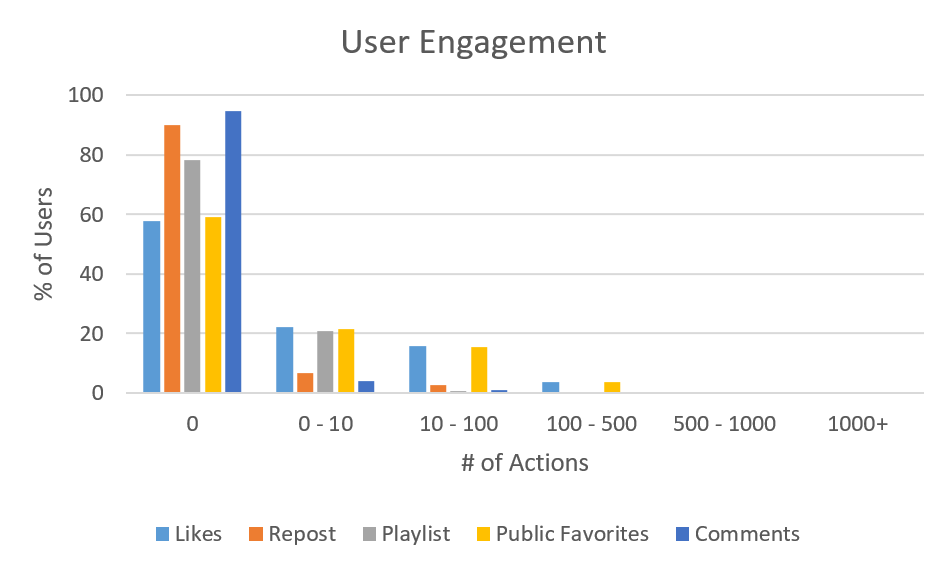
\includegraphics[width=1.0\linewidth]{images/activity_histogram}
\caption{}
\label{fig:activity_histogram}
\end{figure}


\paragraph{Followers, Following, Descriptions \& URLs} We found interesting clusters when analysing the ratio of followers to following. While there was an expected large group of people that had very little followers/followings (39\% of users follow no one; 45\% of users are followed by no one), we found two clusters of users that followed around 250-350 users, but had little to no users following them. Manually inspecting these users, we found multiple spam accounts.
\par To further tighten these clusters, we tried discriminating users by whether or not they provided a Description or a URL. This proved to be beneficial as most  of the spam provides both and as seen in Figure \ref{fig:Following_vs_Followers_w_description_and_url} the spam clusters become more obvious.

\begin{figure}
\centering
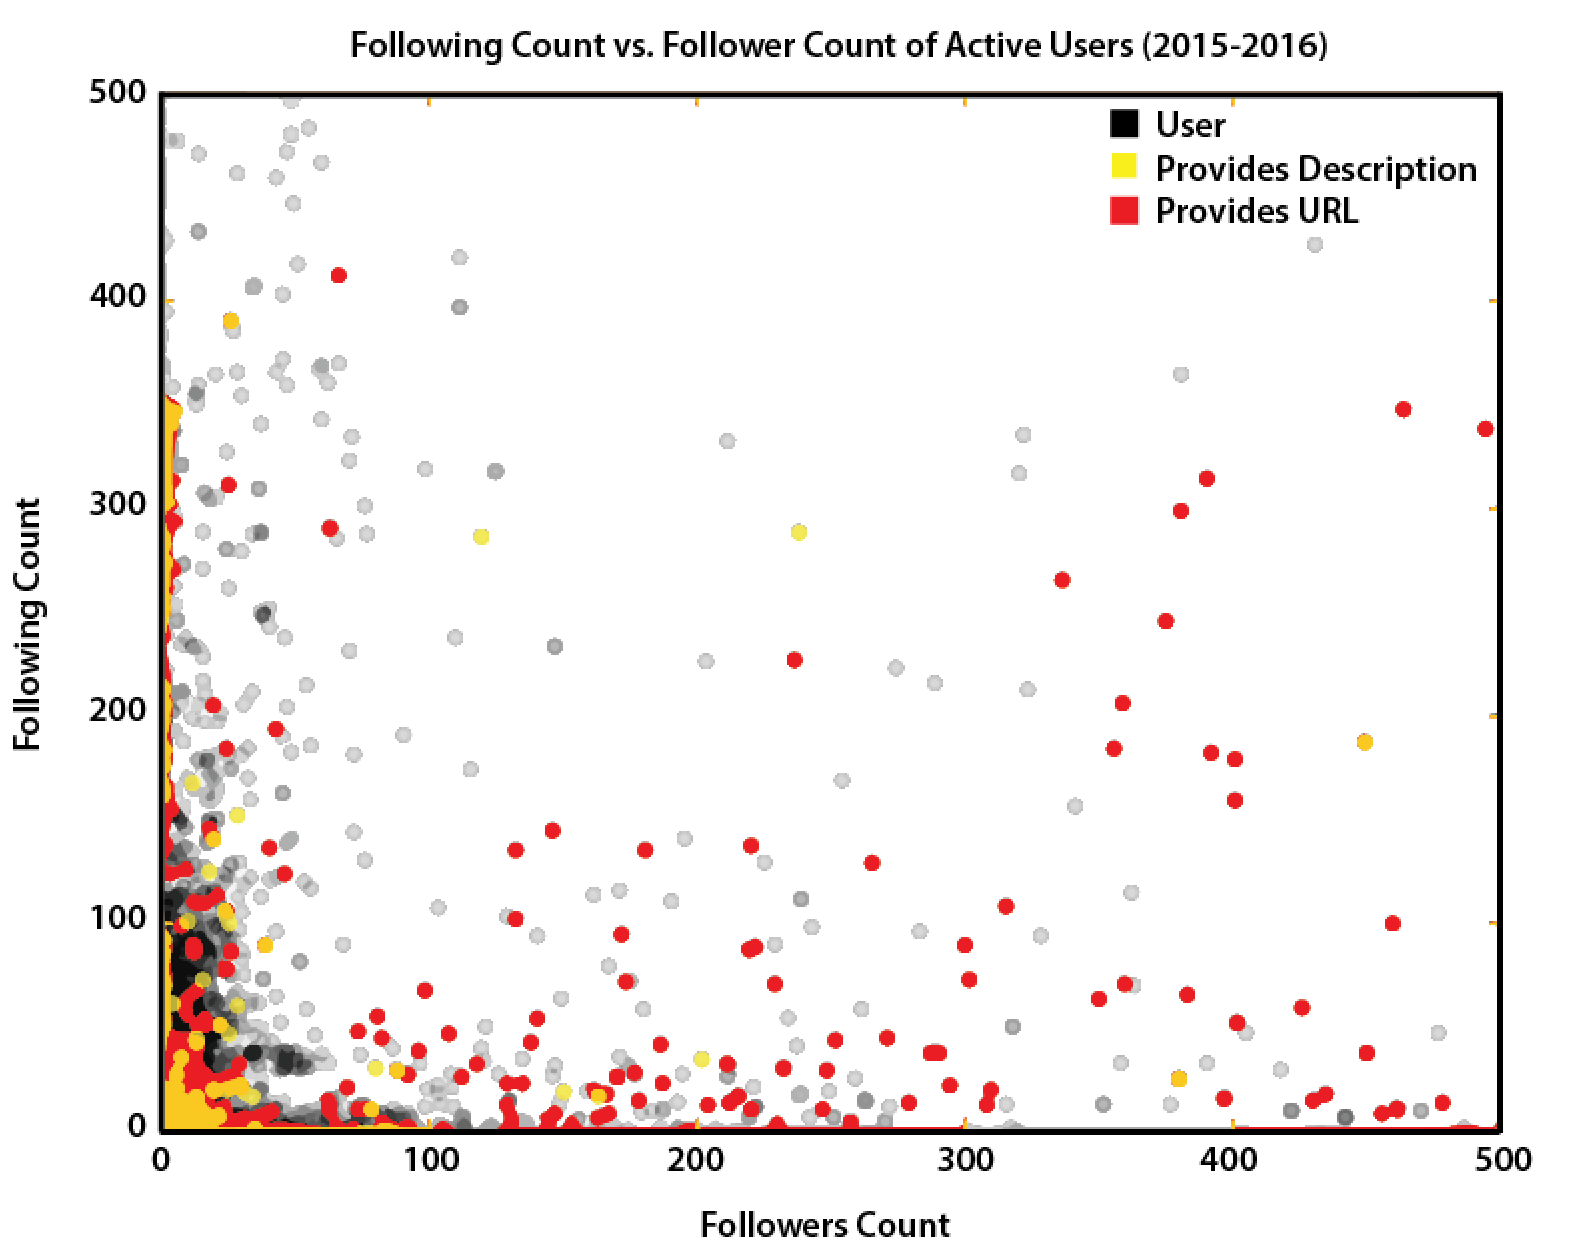
\includegraphics[width=1.0\linewidth]{images/Following_vs_Followers_w_description_and_url}
\caption{}
\label{fig:Following_vs_Followers_w_description_and_url}
\end{figure}

\par We also found that only 0.68\% of users share URLs, and only 0.004\% of them use url shorteners. As such, we manually inspected users using URL shortness and found that it was almost all exclusively spam.

\begin{figure}
	\centering
	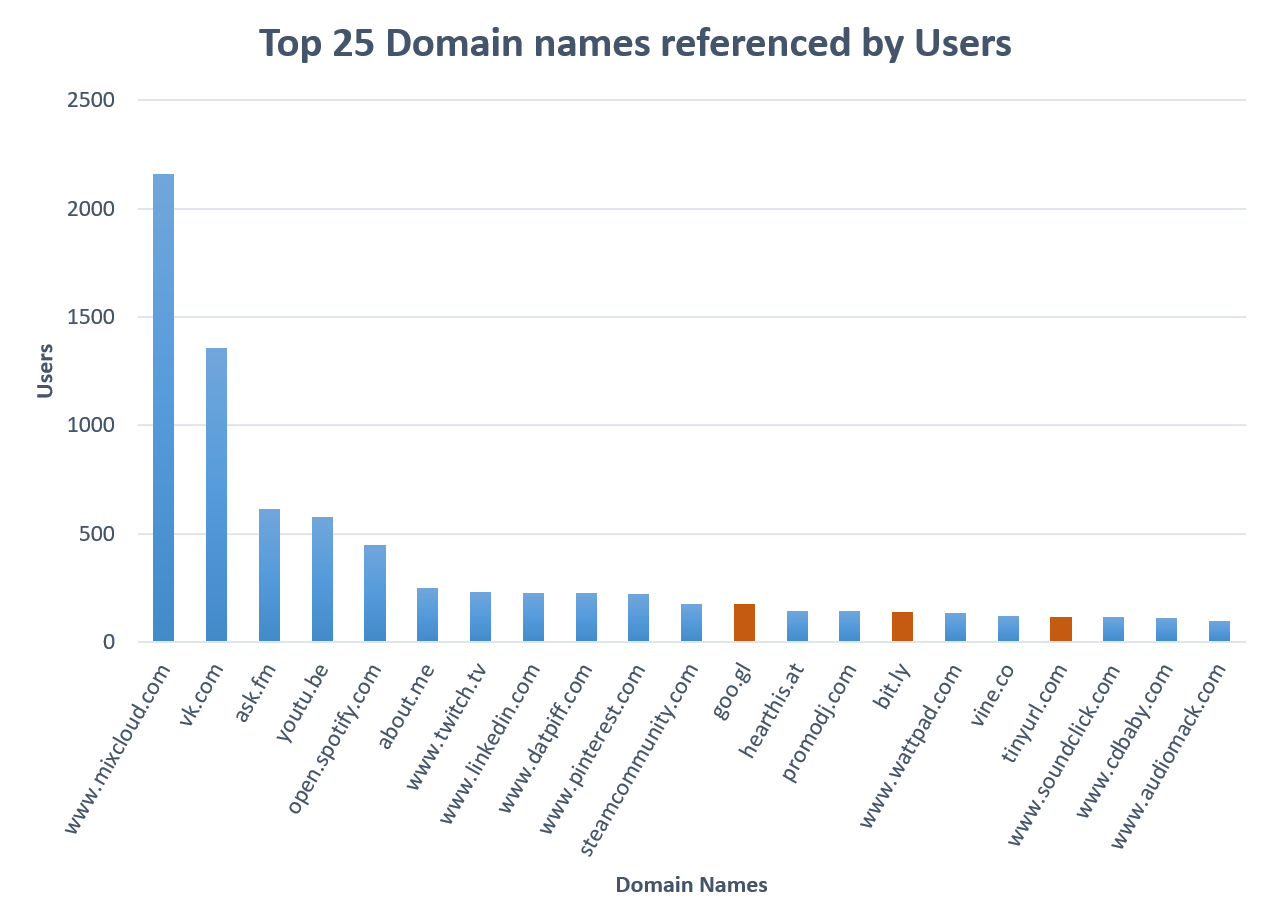
\includegraphics[width=1.0\linewidth]{images/domain_histogram}
	\caption{}
	\label{fig:domain_histogram}
	\end{figure}

\paragraph{Defining Features}
After we had manually visualized the data, understood how users were interacting with the system, and even encountered a few different types of spam, we selected a broad set of Features that could help throughly describe users.

\begin{center}
	\begin{tabular}{ | c | l |}
		\hline
		Feature & Description \\
		\hline
		Followers & \# of users a user is following \\
		Following & \# of following users a user has  \\
		Published & \# of tracks published \\
		URL & Whether user provides a link \\
		ProfaneDesc & \# of profanities in description \\
		ProfacenWeb & \# of profanities in website title \\
		Action & Likes + Reposts + Playlists
		 + Comments + Favorites \\
		Pays & Whether the user pays for Soundcloud \\
		DuplicateDesc & \# of users whit the same description.\\
		DuplicateWeb & \# of users with the same link \\
		ShortenURL & Wether the link point to a url shortner. \\
		\hline
	\end{tabular}
	\newline
	\newline
	\textbf{Table \#2 } - Selected Parameters for both NN using Word Embeddings or Feature Vectors
\end{center}


\section{K-Means Clustering}
\subsection{Methodologies}
\subsection{Classifications}
\subsection{Accuracy in Results}

\section{Neural Network}
In addition to our K-means clustering we wanted to build and train a simple and easy to use service to quickly distinguish spam users in Soundcloud. To do this we built a Neural Network (NN) using the Keras and Tensorflow libraries for Python, and wrapped it around a \textbf{Ruby} web interface that allows users to do quick queries. We are currently hosting this service on www.soundcloud.pw and www.soundcloud.space
\par Our NN is configured as a Feed-Foward NN with 1 hidden layer of 250 ReLU nodes, and an output layer using the sigmoid function as the activation function. We trained it using manually labeled data that we obtained with our Clustering experiments. We made sure that such test cases where in fact well balanced and provided a good mix of different types of users and spam.
\par After training, we tested it against 20,000 randomly chosen users (evenly split between legitimate users and spam), and obtained an accuracy 85\%.


\section{Type of Spam and Origin}
\subsubsection{Pornography Related Spam}
Many of the pornography related spam used URL shorteners that linked to other redirection sites before landing on pornographic websites. The two most common sites where \textit{mrbtrack.com} and \textit{super-goood.ru}; Both which are registered in Russia and are hosted in Russia and Germany respectively. We also found a set of links that followed a similar pattern of 9 random letters and always finished with an African top level domain (e.g \textit{sungzkfpm.ga}).
\subsubsection{``Fake" Users}
We found many users that had identical descriptions and were created within close milliseconds of each other. This types of users seemed to follow a bigger pattern that would slightly randomize the descriptions and choose legitimate looking names, locations, etc. This made these types of users blend easily with real users. However, we still don't know what purpose they serve, as they have no activity and provide no URL or description that would otherwise imply a malicious behaviour.



\section{Future Work}
\textbf{[TODO: Graph Analyis because of spam removal, following non-interactive spam (wtf does it do?),etc,etc.]}

\section{Conclusions}

\end{document}
